\documentclass{article}

\usepackage[utf8]{inputenc}
\usepackage[T1]{fontenc}
\usepackage[italian]{babel}

\usepackage{hyperref, listings, float, graphicx, amsmath, amssymb}
\usepackage{longtable, rotating, listings, booktabs, multicol}
\usepackage[square, sort, comma, numbers]{natbib}
\usepackage[nottoc]{tocbibind}
\usepackage{cleveref, multirow}
\usepackage{lipsum}
\usepackage[dvipsnames]{xcolor}
\usepackage[autostyle=true]{csquotes}

% listing definition

\definecolor{codegreen}{rgb}{0,0.6,0}
\definecolor{codegray}{rgb}{0.5,0.5,0.5}
\definecolor{codepurple}{rgb}{0.58,0,0.82}
\definecolor{backcolour}{rgb}{0.95,0.95,0.92}

\lstdefinelanguage{Turtle}{
    sensitive = true,
    keywords={},
    keywords = [2]{owl:, rdf:, rdfs:, schema:, sh:, xsd:, ex:, id:, idref:, sid:, sidref:,
    usid:, usidref:, lsid:, portsid:, portsidref:, sboterm:},
    keywords = [3]{@prefix, a},
    keywordstyle=\color{backcolour},
    keywordstyle=[2]\color{blue},% for example
    keywordstyle=[3]\color{codepurple},
    numbers=left,
    numberstyle=\scriptsize,
    stepnumber=1,
    numbersep=8pt,
    showstringspaces=false,
    breaklines=true,
    frame=top,
    comment=[l]{\#},
    commentstyle=\color{codegreen}\ttfamily,
    morestring=[b]',
    morestring=[b]" 
}

\lstdefinestyle{mycode}{
    backgroundcolor=\color{backcolour},   
    commentstyle=\color{codegreen},
    keywordstyle=\color{magenta},
    numberstyle=\tiny\color{codegray},
    stringstyle=\color{codepurple},
    basicstyle=\ttfamily\footnotesize,
    breakatwhitespace=false,         
    breaklines=true,                 
    captionpos=b,                    
    keepspaces=true,                 
    numbers=left,                    
    numbersep=5pt,                  
    showspaces=false,                
    showstringspaces=false,
    showtabs=false,                  
    tabsize=2
}

\lstset{style=mycode}

\title{SBML2SHACL}

\author{Edoardo De Matteis}

\begin{document}
\maketitle
\tableofcontents

\clearpage
\section{Logiche Descrittive} \label{sec:dl}
La logica del primo ordine (FOL) aggiunge espressività alla logica proposizionale introducendo predicati, funzioni e quantificatori e permettendo di modellare eventi dinamici nel tempo al prezzo di un'inferenza semidecidibile, data infatti una knowledge base KB e una formula $\alpha$ è sempre possibile scrivere un algoritmo che risponda affermativamente se $KB \models \alpha$ ma se $KB \nvDash \alpha$ l'esecuzione potrebbe non terminare. 

Le \textbf{description logics} (DL) ~\cite{dl:handbook} sono una famiglia di linguaggi formali per rappresentazione della conoscenza spesso più espressivi della logica proposizionale, che è priva di quantificatori e fa uso di proposizioni dichiarative, ma meno della logica del primo ordine, nella quale si fa uso di quantificatori, predicati, funzioni e variabili; per alcuni di questi linguaggi esistono algoritmi d'inferenza corretti e completi, più il linguaggio diventa espressivo più è difficile che l'inferenza sia decidibile. 

La sintassi delle DL è fatta in modo tale da rendere facile la modellazione di definizioni e proprietà di categorie (collezioni di "oggetti" utilizzate per la rappresentazione di conoscenza su larga scala) tramite operazioni insiemistiche piuttosto che con una caratterizzazione logica 

Se in FOL abbiamo \textbf{costante}, \textbf{predicato unario} e \textbf{predicato binario} nelle DL si ha rispettivamente \textbf{individuo}, \textbf{concetto} e \textbf{ruolo}; se in FOL si parla di statement nelle DL si parla di descrizioni. Le descrizioni elementari sono descrizioni composte da concetti e ruoli atomici e combinandole tra loro si ottenegono descrizioni complesse, le descrizioni di concetti nella logica descrittiva $ \mathcal{AL} $ si ottengono secondo la seguente sintassi, si adotta la convenzione per cui $ A $ rappresenta concetti atomici e $ C, D $ descrizioni di concetti.

\begin{table}[h!] 
    \centering
    \begin{tabular}{r c l l}
        $ C, D $ & $ \rightarrow $ & $ \ \ A $ & (concetto atomico) \\
        & & $ | \ \top $ & (concetto universale) \\
        & & $ | \ \bot $ & (concetto nullo) \\
        & & $ | \ \neg A $ & (negazione atomica) \\
        & & $ | \ C \sqcap D $ & (intersezione) \\
        & & $ | \ \forall R.C $ & (restrizione di valore) \\
        & & $ | \ \exists R.\top $ & (quantificazione esistenziale limitata) \\
    \end{tabular}
\end{table}

Come in FOL un'interpretazione $I$ consiste di un insieme non vuoto $\Delta^{I}$, il dominio d'interpretazione, e di una funzione di interpretazione che assegna ad ogni concetto atomico $A$ un insieme $A^{I} \subseteq \Delta^{I}$ e ad ogni ruolo atomico $R$ una relazione binaria $R^{I} \subseteq \Delta^{I} \times \Delta^{I}$. Tramite le definizioni induttive seguenti è possibile estende la funzione di interpretazione per le descrizioni di concetti.

\begin{gather*}
    \top^{I} = \Delta^{I} \\
    \bot^{I} = \emptyset \\
    \neg A^{I} = \Delta^{I} \setminus A^{I} \\
    (C \sqcap D)^{I} = C^{I} \cap D^{I} \\
    (\forall R.C)^{I} = \{ a \in \Delta^{I} | \forall b.(a,b) \in R^{I} \rightarrow b \in C^{I} \} \\
    (\exists R.\top)^{I} = \{ a \in \Delta^{I} | \exists b.(a,b) \in R^{I} \} \\
\end{gather*}

Dal momento che le DL sono una famiglia possiamo definire una logica descrittiva ~\cite[Appendix 1]{dl:handbook} componendo vari frammenti che ne indicano l'espressività, ad esempio possiamo estendere $ \mathcal{AL} $ con i costrutti in tabella \ref{tab:extend_DL}, nella tabella \ref{tab:fragments_DL} è possibile consultare il nome di alcuni frammenti cui sono propri determinati costrutti.

\begin{table}[h!t] 
    \centering
    \caption{Paronamica di frammenti di DL che ci permettono di avere la stessa espressività della FOL.}
    \label{tab:extend_DL}
    \begin{tabular}{c c c}
        \textbf{Costrutto} & \textbf{Sintassi} & \textbf{Semantica} \\
        \hline
        Top & $\top$ & $\Delta^{\mathcal{I}}$ \\
        Bottom & $\bot$ & $\emptyset$ \\
        Intersezione & $C \sqcap D$ & $C^{\mathcal{I}} \cap D^{\mathcal{I}}$ \\
        Unione & $C \sqcup D$ & $C^{\mathcal{I}} \cup D^{\mathcal{I}}$ \\ 
        Negazione & $\neg C$ & $\Delta^{\mathcal{I}} \setminus C^{\mathcal{I}}$ \\
        Restrizione & $\forall R.C$ & 
        $\{ a \in \Delta^{\mathcal{I}} | \forall b.(a,b) \in R^{\mathcal{I}} \rightarrow b \in C^{\mathcal{I}} \}$ \\
        Esistenziale & $\exists R.C$ & 
        $\{ a \in \Delta^{\mathcal{I}} | \exists b.(a,b) \in R^{\mathcal{I}} \land b \in C^{\mathcal{I}} \}$ \\
        \hline
    \end{tabular}
\end{table}

Per comprendere meglio le DL è utile vedere una corrispondenza tra alcuni costrutti in FOL e nelle DL (tabella \ref{tab:DL_FOL}) e vedere alcune descrizioni d'esempio. 

\begin{table}[h!t]
    \centering
    \caption{Corrispondenza DL e FOL.}
    \label{tab:DL_FOL}
    \begin{tabular}{c c}
        \hline 
        \textbf{FOL} & \textbf{DL} \\
        \hline
        $ A(x) $ & $ A $ \\
        $ C(a) $ & $ C(a) $, $ a:C $ \\
        $ \neg C(x) $ & $ \neg C $ \\
        $ C(x) \land D(x) $ & $ C \sqcap D $ \\
        $ C(x) \lor D(x) $ & $ C \sqcup D $ \\
        $ \forall x . C(x) \rightarrow D(x) $ & $ C \sqsubseteq D $ \\
        $ R(a,b) $ & $ R(a,b) $, $ (a,b):R $ \\
        $ \forall x, y . R(x,y) \rightarrow S(x,y) $ & $ R \sqsubseteq S $ \\
        $ \exists y . R(x,y) \land C(y) $ & $ \exists R.C $ \\
        $ \forall x, y, z . R(x,y) \rightarrow R(y,z) \rightarrow R(x,z) $ & $ R \circ R \sqsubseteq R $ \\
        $ A \leftrightarrow B $ & $ A \equiv B $ \\
        \hline
    \end{tabular}
\end{table}

Siano $ \textbf{Uomo} $, $ \textbf{Mortale} $ concetti atomici, $ \underline{\textrm{allievoDi}} $ un ruolo atomico e $ Socrate $, $ Platone $ individui. 
\begin{itemize}
    \item Socrate è un uomo. 
    \begin{equation*}
         Socrate:\textbf{Uomo}
    \end{equation*}
    \item Ogni uomo è mortale.
    \begin{equation*}
        \textbf{Uomo} \sqsubseteq \textbf{Mortale}
    \end{equation*}
    \item Se ogni uomo è mortale e Socrate è un uomo allora ogni uomo è mortale.
    \begin{equation}
        \label{eq:subsumption}
        [(\textbf{Uomo} \sqsubseteq \textbf{Mortale}) \sqcap Socrate:\textbf{Uomo}] \sqsubseteq Socrate:\textbf{Mortale}
    \end{equation}
    \item Platone è allievo di Socrate.
    \begin{equation*}
        (Platone, Socrate):\underline{\textrm{allievoDi}}
    \end{equation*}
\end{itemize}

\begin{table}[h!t] 
    \centering
    \caption{Alcuni simboli di DL con associati i costrutti caratteristici.}
    \label{tab:fragments_DL}
    \begin{longtable}{p{0.1\textwidth}p{0.3\textwidth}p{0.5\textwidth}}
        \textbf{Simbolo} & \textbf{Costrutti} & \textbf{Esempio}  \\
        \hline
        $\mathcal{AL}$ & 
        Negazione atomica, intersezione di concetti, restrizione universale, quantificazione esistenziale limitata & 
        $ \textbf{Gatto} \equiv \textbf{Domestico} \sqcap \textbf{Felino} $ \\
        \hline
        $\mathcal{C}$ & 
        Classe di espressioni complesse ottenute combinando operatori quali la relazione di sottoclasse, equivalenza, congiunzione, disgiunzione, negazione, restrizioni, tautologie e contraddizioni & 
        $ \textbf{Gatto} \equiv \textbf{Felino} \sqcap \neg (\textbf{Leone} \sqcup \textbf{Tigre}) $ \\
        \hline
        $\mathcal{S}$ & $ \mathcal{ALC} $ con ruoli transitivi &
        $ \textrm{\underline{antenatoDi}} \circ \textrm{\underline{antenatoDi}} \sqsubseteq \textrm{\underline{antenatoDi}} $ \\
        \hline
        $\mathcal{E}$ & Quantificazione esistenziale completa & 
        $ \exists \textrm{\underline{mangiatoDa}}.\textbf{Insetto} $ \\
        \hline
        $\mathcal{U}$ & Unione di concetti & $ \textbf{Animale} \equiv \textbf{Cane} \sqcup \textbf{Gatto} $ \\
        \hline
        $\mathcal{H}$ & Gerarchia di ruoli & $ \textrm{\underline{mangiatoDa}} \sqsubseteq \textrm{\underline{predaDi}} $ \\
        \hline
        $\mathcal{O}$ & Classi enumerate di oggetti & $ \textbf{Italia} \equiv \{ \textbf{Nord}, \textbf{Centro}, \textbf{Sud} \} $ \\
        \hline
        $\mathcal{I}$ & Ruoli inversi & $ \textrm{\underline{predatoreDi}} \equiv \textrm{\underline{predaDi}}^{-} $ \\
        \hline
        $\mathcal{Q}$ & Restrizione di cardinalità qualificata & $ \textbf{Gatto} \sqsubseteq  \ = \! 4\textrm{\underline{haGambe}} $ \\
        \hline
        $\mathcal{(D)}$ & Uso di tipi di dati, sue proprietà o valori &  \\
        \hline
    \end{longtable}
\end{table}

Dal momento che nelle DL si eseguono operazioni insiemistiche non si parla propriamente di inferenza ma di sussunzione (subsumption): $C \sqsubseteq D$ equivale in FOL a $C \rightarrow D$, similmente a quanto avviene nel model checking in logica proposizionale $\alpha \models \beta \longleftrightarrow M(\alpha) \subseteq M(\beta)$ - la funzione $M(\phi)$ data una formula $\phi$ ne restituisce l'insieme dei modelli - e per il teorema di deduzione $\alpha \models \beta  \longleftrightarrow \alpha \rightarrow \beta$. L'equazione \ref{eq:subsumption} è un esempio di sussunzione.

Le DL si basano su un'interfaccia "tell and ask" e si fanno sussunzioni analizzando TBox e ABox della KB: nella TBox si danno le definizioni dei concetti e si forma una conoscenza intensionale, ad esempio è qui che sarà presente $ \textbf{Gatto} \equiv \textbf{Domestico} \sqcap \textbf{Felino} $; quando si costruisce una TBox l'operazione base di ragionamento è la \textit{classification} e consiste nel posizionare il concetto appena definito in una giusta gerarchia rispetto ai concetti già presenti nella TBox, ciò è ottenuto verificando la sussunzione tra il concetto preso in esame e ogni altro concetto nella TBox. In questo progetto la TBox corrisponde al file \texttt{shapes.ttl}, la definizione di un concetto corrisponde infatti alla definizione di una shape.

Nell'ABox invece sono presenti le affermazioni su individui (membership assertions), si definsice quindi una conoscenza estensionale del dominio di interesse: è qui che va ad esempio la descrizione $ Silvestro:\textbf{Gatto} $. La principale operazione di ragionamento in un'ABox è l'\textit{instance checking} nel quale si verifica che un individuo sia un'istanza di un dato concetto; altre operazioni svolte sono le seguenti che comunque non sono altro che casi particolari di \textit{instance checking}. 
\begin{itemize}
    \item \textit{knowledge base consinstency} con la quale si verifica che per ogni concetto esista almeno un individuo istanziato. 
    \item \textit{realization} con la quale si trova il concetto più specifico del quale un individuo è istanza. 
    \item \textit{retrieval} col il quale dato un concetto si trovano tutti gli individui che ne sono istanza.
\end{itemize}
Il file \textit{output.ttl} generato dai parser \texttt{parser.py} e \texttt{extended\_parser.py} corrisponde all'ABox, quando si verifica la sua correttezza rispetto alla TBox \texttt{shapes.ttl} con \texttt{shacl\_verifier.py} si eseguono le sussunzioni alla base delle operazioni di ragionamento sopra descritte .

\subsection{RDF} \label{sec:rdf}
Il \textbf{Resource Description Framework (RDF)} ~\cite{rdf} è una famiglia di specifiche definite dal World Wide Web Consortium (W3C) utilizzate per la modellazione di informazioni implementate come risorse web. RDF è simile ad altri approcci classici come database relazionali o logiche descrittive nei quali si hanno affermazioni sulle risorse sotto forma di triple soggetto-predicato-oggetto; il soggetto è la risorsa stessa e il predicato esprime una relazione tra soggetto e oggetto.

Se ad esempio volessimo esprimere il concetto "il cielo è blu" avremmo:
\begin{itemize}
    \item [] \textbf{soggetto}: "il cielo"
    \item [] \textbf{predicato}: "è di colore"
    \item [] \textbf{oggetto}: "blu"
\end{itemize}

Contrariamente all'approccio object oriented entità-attributo-valore in cui avremmo un oggetto "cielo" con attributo "colore" di valore "blu". Come si può vedere nell'\href{https://book.validatingrdf.com/bookHtml008.html}{immagine} \ref{fig:graph} un insieme di triple rappresenta intrinsecamente un grafo: una rappresentazione decisamente conveniente ma spesso nella pratica un modello RDF è mantenuto come database relazionale (chiamato Triplestore o Quad store).

\begin{figure}[h!t]
    \caption{Un modello RDF è un grafo.}
    \label{fig:graph}
    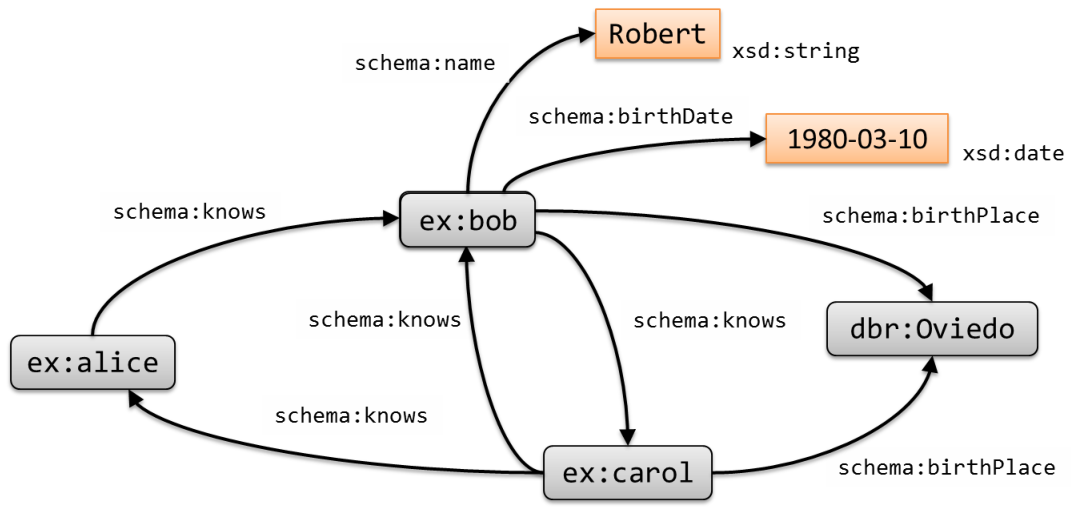
\includegraphics[scale=0.3]{images/RDFGraph.png}
    \centering
\end{figure}

L'ABox è definita in RDF (nello specifico Turtle in quanto è il linguaggio RDF scelto) che è meno espressivo delle DL ~\cite[Logic for the semantic web, 2.4]{logic:computational}, nella tabella \ref{tab:DL_RDF} si vede come sia possibile esprimere alcune espressioni RDF con le logiche descrittive: 

\begin{table}[h!t]
    \centering
    \caption{Traduzione da RDF a DL.}
    \label{tab:DL_RDF}
    \begin{tabular}{c c}
        \hline 
        \textbf{RDF} & \textbf{DL} \\
        \hline
        $ x $ \texttt{rdfs:type} $ A $ & $ A(x) $ \\
        $ x P y $ & $ P(x,y) $ \\
        $ A $ \texttt{rdfs:subClassOf} $ B $ & $ A \sqsubseteq B $ \\
        $ P $ \texttt{rdfs:domain} $ A $ & $ \exists P \sqsubseteq A $ \\
        $ A $ \texttt{rdfs:range} $ B $ & $ \exists P^{-} \sqsubseteq A $ \\
        $ P $ \texttt{rdfs:subPropertyOf} $ Q $ & $ P \sqsubseteq Q $ \\
        \hline
    \end{tabular}
\end{table}

\subsection{SHACL} \label{sec:shacl}
\textbf{Shapes Constraint Language (SHACL)} ~\cite{shacl} è una specifica del W3C per la verifica di informazioni sotto forma di grafi rispetto ad un insieme di vincoli, include anche il linguaggio di query \textbf{SPARQL Protocol and RDF Query Language (SPARQL)} ~\cite{sparql}.
Il processo di verifica prende in input un grafo contenente le dichiarazioni delle shape ovvero le definizioni cui i nodi, le istanze, dovranno essere verificati; in input si può avere qualsiasi formato RDF e in questo progetto si userà Turtle; SHACL è diretto discendente di OWL ~\cite{shacl:owl} il quale è stato progettato basandosi su RDF e sulle description logics, è composto infatti da \textit{RDF-Based semantics} e \textit{direct semantics} rispettivamente e la seconda è più espressiva della prima ~\cite[7]{rdf:semantics} ~\cite[Logic for the semantic web, 3.2]{logic:computational}. La TBox come l'ABox è definita in Turtle quindi RDF, il ruolo di SHACL è quello di verificare tramite inferenza la consistenza di TBox e ABox: è qui che avviene la vera fase di ragionamento, in questo progetto è svolta dall'agente razionale \texttt{shacl\_verifier.py}.

SHACL corrisponde ad una logica descrittiva molto estesa - $\mathcal{ALCOIQ(\circ)}$ - che è corretta, non completa, senza garanzie di terminazione e NEXPTIME-hard; le premesse non sembrano ottimistiche ma è possibile rendere meno espressivo il linguaggio per ottenerere inferenze decidibili. Escludendo la composizione di ruoli $\circ$ si ha $\mathcal{SROIQ}$ per la quale esiste un algoritmo d'inferenza corretto, non completo, decidibile e NEXPTIME-hard; escludendo anche la possibilità di esprimere ruoli inversi si ottiene la DL $\mathcal{ALCOQ}$ che è sound, completa, decidibile e PSPACE-complete e dal momento che NP $\subseteq$ PSPACE $\subseteq$ EXPTIME si ha un netto miglioramento. Questi risultati sono stati ottenuti grazie ad un navigator online per logiche descrittive ~\cite{dl:complexity}.

\clearpage
\section{Caso di studio}

\subsection{SBML}
\textbf{Systems Biology Markup Language (SBML)} ~\cite{sbml} è un formato di rappresentazione basato su XML per la modellazione di processi biologici e chimici. Non è un linguaggio bensì una \textit{lingua franca} tra tool che utilizzano formati di rappresentazione differenti e ad oggi è \textit{de facto} uno standard per i modelli computazionali in biologia. 

Ai fini di questo progetto distinguiamo due differenti SBML:
\begin{itemize}
    \item \textbf{SBML Level 3} ~\cite{sbml:core}. La specifica del \textit{Core} che offre le funzionalità base di SBML, in questo documento lo si indica come "SBML 3".
    \item \textbf{Hierarchical Model Composition} ~\cite{sbml:hierarcical}. Noto come "comp" (namespace del package e quindi parola chiave in XML) questo package offre la possibilità di include modelli annidati permettendo allo sviluppatore ed eventuali tool di:
    \begin{enumerate}
        \item Scomporre modelli troppo grandi in modelli più piccoli per ridurne la complessità.
        \item Avere istanze multiple di un modello - precedentemente definito - all'interno di altri modelli, evitando ripetizione di codice. 
        \item Creare librerie di codice riusabile e modelli considerati corretti. 
    \end{enumerate}
    In questo documento lo si indica come "Extended SBML". 
\end{itemize}

\subsection{Obiettivi}

Lo scopo di questo progetto, sotto la guida dei Professor Mancini e del Professor Tronci, è quello di convertire automaticamente una specifica SBML in SHACL. A tal fine il problema è stato diviso in tre fasi:

\begin{enumerate}
    \item Modellare in SHACL un sottoinsieme di costrutti che definiscono SBML . 
    \item Scrivere un parser che traduca una specifica SBML in SHACL.
    \item Scrivere un parser che traduca una specifica SHACL in SBML.
\end{enumerate}

Si assume a priori che i file SBML in input siano corretti, la \href{http://sbml.org/Facilities/Validator}{verifica} è eseguibile online. Per il corretto funzionamento del codice inoltre è necessario il download del package Python \textit{rdflib}.

\clearpage
\section{Modellazione}

In questa prima fase si è scelto un sottoinsieme di SBML 3.2 più i costrutti in Extended SBML e ne è stato formalizzato un modello. Nella tabella ~\ref{tab:modellazione} vengono descritti i principali costrutti, sono state volontariamente omesse shape quali \texttt{listOf*} il cui significato è intuitivo e avrebbero solo reso la tabella meno leggibile, in ogni caso è possibile consultare ulteriormente il diagramma \texttt{diagram.png}, mostrato anche in figura \ref{fig:diagram}, e il file delle shape \texttt{shapes.ttl}.

\begin{longtable}{p{.4\textwidth}p{.5\textwidth}}
    \textbf{Entità} & \textbf{Descrizione} \\
    \hline
    \multicolumn{2}{c}{SBML 3.2} \\
    \hline
    SBase & Classe astratta superclasse di ogni altra classe. Per quanto in SBML sia considerata a tutti gli effetti un tipo, poiché non esistono attributi di tipo SBase a questa classe si riserva un trattamento differente rispetto ai tipi composti quali ID, SId, etc \dots che sono state omesse dal diagramma ma sono comunque presenti nel file \texttt{shapes.ttl}. \\ 
    \hline
    Sbml & Ogni file SBML ha un'etichetta con tag \texttt{sbml}, data la sua obbligatorietà ed unicità è possibile costruire grafi SHACL composti da multipli modelli SBML ed esplorarli radicando l'albero in Sbml, è importante specificare che questo nuovo modello composto non sarà legale in SBML e non si dà alcuna garanzia nella fase di riconversione in SBML. Il costrutto Sbml ammette altri attributi oltre quelli noti, siccome in SHACL ho necessità di conoscerne il tipo è stata persa questa possibilità.\\
    \hline
    Model & Rappresenta il modello, se ne può avere più di uno come detto sopra nonostante SBML non lo permetta. \\
    \hline
    Unit & Definisce un'unità di misura definita dall'utente, in SBML sono definite delle unità base (i.e. le unità del SI e altre scelte dagli sviluppatori di SBML) e combinandole opportunamente tra loro è possibile definire nuove unità di misura (e.g l'accelerazione $\frac{m}{s^{2}}$ che altro non è se non $m^{1}s^{-2}$). Nel modello in \texttt{shapes.ttl} le unità base (kind) sono trattate come normalissime unità di misura, in SBML non è concesso avere come attributo kind un'unità di misura che non sia base e questa libertà non genera problemi. \\
    \hline 
    Compartment & Rappresenta un insieme di entità biologiche. \\
    \hline
    Species & Rappresenta un'entità biologica. \\
    \hline
    Parameter & In SBML si possono definire parametri sia locali che globali, il modello presentato in queso progetto non implementa la località quindi i parametri sono sempre globali e in Model l'attributo \texttt{ListOfParameters} ha moltiplicità $[0,n]$ piuttosto che $[0,1]$. \\  
    \hline 
    \multicolumn{2}{c}{Extended SBML} \\
    \hline
    ExternalModelDefinition &  Necessario per importare modelli esterni. \\
    \hline
    ModelDefinition & Questo costrutto fornisce la definizione di un modello. \\ 
    \hline
    Submodel & L'istanza di una ModelDefinition è rappresentata da un Submodel, si ha quindi un modello dentro ad un altro modello. Durante la fase di test per extended SBML non ho usato esempi scaricati da Biomodels perché la gerarchia non veniva rappresentata tramite il costrutto Submodel ma con un attributo \texttt{outer} in Compartment, con il Professor Tronci si è ritenuto fosse meglio attenersi allo standard W3C. \\ 
    \hline
    Port & Una port permette allo sviluppatore di definire come ci si deve interfacciare con un modello, per quanto non siano vincolanti di norma è preferibile seguire le indicazioni dello sviluppatore. \\ 
    \hline
    Deletion & Non è detto che i modelli importati abbiano solo ed esclusivamente componenti desiderabili e con una deletion è possibile ignorare quelli indesiderati. \\
    \hline
    Replacement & Tramite questo costrutto è possibile sostituire una componente con un'altra, ogni riferimento alla prima ora punta alla seconda. A causa di Replacement sono presenti più parser: il primo \texttt{parser.py} esplora il file XML come una lista ed \texttt{extended\_parser.py} come un albero. \\
    \hline
    SBaseRef & Port, Deletion, Replacement e Submodel utilizzano dei riferimenti, SBaseRef similmente a SBase offre alle proprie sottoclassi degli attributi comuni a tutte. \\
    \hline

    \caption{Modellazione SHACL}
    \label{tab:modellazione}
\end{longtable}

Prendiamo d'esempio il file SBML dato in input al parser \texttt{example.xml}, l'output \texttt{output.ttl}, il file \texttt{shapes.ttl}, il diagramma \texttt{diagram.png} e vediamo come viene popolata l'ABox rispetto al costrutto \texttt{model}. Nel listato \ref{lst:input_model} è stata isolata la parte che riguarda il modello dal file in input, gli attributi presenti nell'etichetta sono \texttt{id}, \texttt{metaid} e \texttt{name}: può essere verificato sia nel diagramma che nel file delle shape, nel listato \ref{lst:shapes_model} è stata isolata la parte relativa al solo costrutto model. Attributo e valore sono quindi tradotti in Turtle rispettivamente in predicato e oggetto, lo si può vedere nel listato \ref{lst:output_model}; lo stesso viene fatto anche per le relazioni con altre entità ove \texttt{model} potrà essere soggetto o oggetto. 

\lstinputlisting[language=xml,linerange={3-18},firstnumber=3,caption={Sezione del modello isolata dal file di input \texttt{example.xml}},label={lst:input_model}]{../examples/input/example.xml}

\lstinputlisting[language=Turtle, caption={Sezione del modello isolata nel file di output \texttt{output.ttl}}, label={lst:output_model}, numbers=none, linerange={225-231,247-247,262-262} ]{../examples/output/output.ttl}

\lstinputlisting[language=Turtle,linerange={294-395},firstnumber=294,caption={Shape model in \texttt{shapes.ttl}},label={lst:shapes_model}]{../project/model/shapes.ttl}

\begin{sidewaysfigure}
    \caption{Modellazione SBML}
    \label{fig:diagram}
    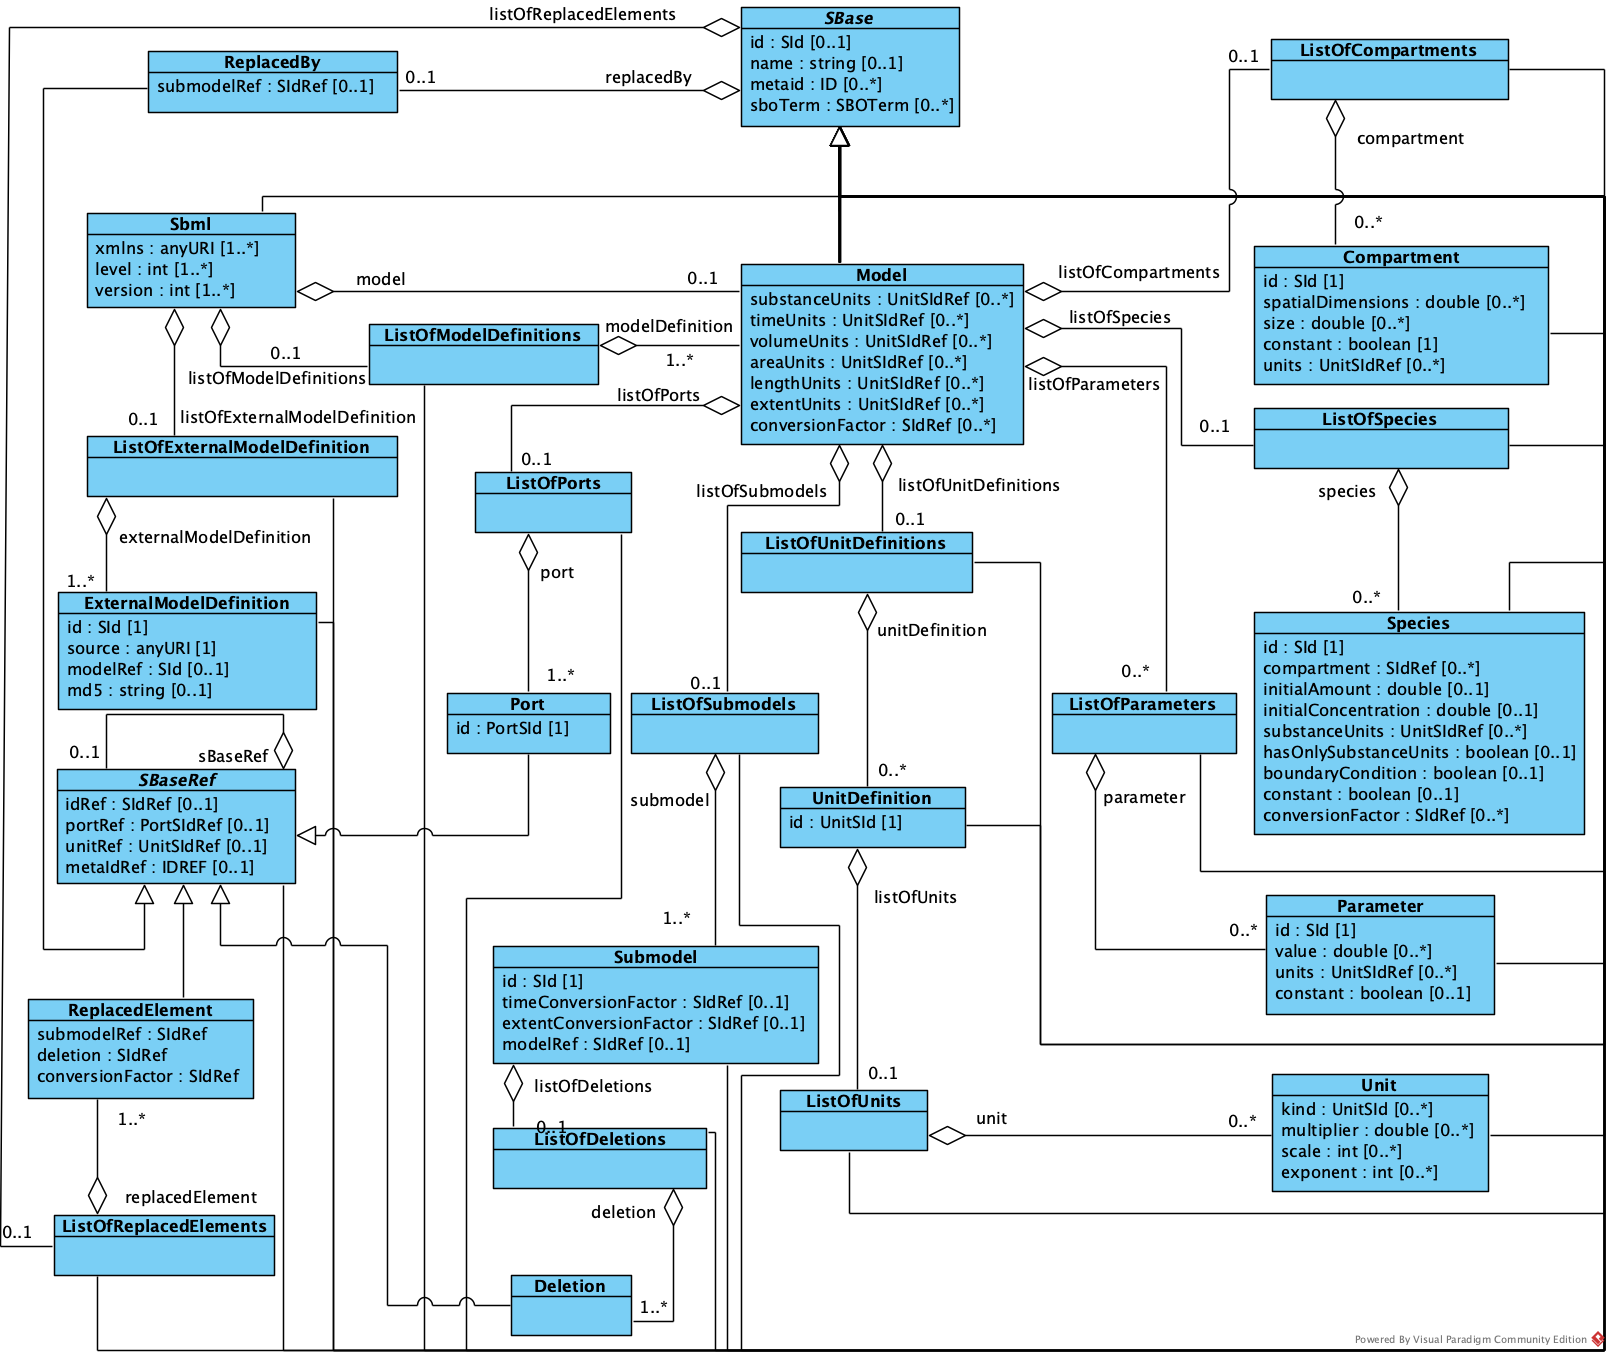
\includegraphics[scale=0.6]{images/diagram.png}
\end{sidewaysfigure}

\clearpage
\section{Parsing da SBML a SHACL}

In questa seconda fase dato uno o più file SBML in input li si traduce in SHACL tramite un parser e si verifica la correttezza dell'output tramite il file \texttt{shacl\_verifier.py}. Come già detto si hanno due parser: \texttt{parser.py} è la prima versione e non supporta Extended SBML contrariamente a \texttt{extended\_parser.py} che è la versione finale. 

In \texttt{parser.py} si riescono a tradurre senza problemi file in SBML 3.2 ma poiché il file XML viene letto come una lista di etichette risulta macchinoso (ammesso e non concesso sia possibile) fare riferimento all'etichetta padre di una sostituzione o una cancellazione. Il problema non si presenta in \texttt{extended\_parser.py} dato che il file XML viene esplorato come un albero, questa seconda versione è inoltre più breve (444 righe anziché 932) ed è più facilmente estendibile. Questo parser infatti legge qualsiasi tag del file XML e associa ogni attributo al rispettivo valore, ho comunque imposto dei controlli per evitare questo comportamento dato che avrebbe solo rallentato la fase di verifica. Inoltre è più veloce come si può vedere in tabella ~\ref{tab:performance}: il calcolo delle performance è basato sull'esecuzione di \texttt{test.sh}, sono stati scaricati da \href{https://www.ebi.ac.uk/biomodels/}{Biomodels} i 18 modelli SBML presenti nella cartella \texttt{examples/input/biomodel} e di seguito elencati, in \texttt{test.sh} i parser prendono in input due file così da verificare la correttezza della costruzione di un grafo a partire da più modelli e allo stesso tempo si ha un numero più consistente di test ovvero 324. 

\begin{multicols}{2}
    \begin{enumerate}
        \item BIOMD0000000087.xml
        \item BIOMD0000000105.xml
        \item BIOMD0000000399.xml
        \item BIOMD0000000474.xml
        \item BIOMD0000000476.xml
        \item BIOMD0000000559.xml
        \item BIOMD0000000562.xml
        \item BIOMD0000000619.xml
        \item BIOMD0000000624.xml
        \item BIOMD0000000705.xml
        \item BIOMD0000000706.xml
        \item MODEL1012110001.xml
        \item MODEL1012220002.xml
        \item MODEL1012220003.xml
        \item MODEL1012220004.xml
        \item MODEL1112260002.xml
        \item MODEL1812100001.xml
        \item MODEL3632127506.xml
    \end{enumerate}
\end{multicols}

\begin{table}[h!t] 
    \centering
    \begin{longtable}{p{0.5\textwidth}p{0.3\textwidth}}
        \textbf{File} & \textbf{Time (m)} \\
        \hline
        %parser.py & 52.90 & 2445.38 & 42:54.54 & 97 \% \\
        parser.py & 42:54.54 \\
        %extended\_parser.py & 38.07 & 1003.51 & 17:35.19 & 98 \% \\
        extended\_parser.py & 17:35.19 \\
        \hline
    \end{longtable}
    \caption{Risultati ottenuti eseguendo \texttt{time ./test.sh} su macOS Catalina 10.15.6 con processore Intel Core i5 1.6 GHz Dual-Core.}
    \label{tab:performance}
\end{table}

Nella sottocartella \texttt{custom} invece vi sono file d'esempio forniti direttamente dal W3C per Extended SBML, potranno essere usati solo per verificare \texttt{extended\_parser.py}. In Biomodels per esprimere una gerarchia tra compartment si fa uso di un attributo \texttt{outer} e non di sottomodelli come nella specifica del W3C.

%\clearpage
\section{Parsing da SHACL a SBML}
Nella terza e ultima fase si esegue la controprova della precedente ovvero si traduce il file di istanze SHACL ottenuto in un file SBML e ci si attende che venga modellata la stessa conoscenza, il file in output non sarà necessariamente uguale a quello di input poiché privo di eventuali costrutti non modellati, è importante notare che è possibile tradurre solo ed esclusivamente delle specifiche Turtle, SHACL è più espressivo di SBML quindi non è sempre possibile ottenere un modello in XML a partire da una specifica SHACL. 

Nella cartella \texttt{query} sono presenti tre file:

\begin{itemize}
    \item \texttt{query.py}: Permette di interrogare il modello con query SPARQL, la query deve essere scritta direttamente nel codice perché gli argomenti della print variano in base alla query.
    \item \texttt{ttl2sbml.py}: Il parser da SHACL a SBML.
    \item \texttt{ttl2xml}: Converte un file di istanze Turtle in XML, una query e un file XML possono esprimere la stessa conoscenza: una tripla \texttt{<subject> <predicate> <object>} si può tradurre in XML nelle etichette \texttt{<subject> <predicate> <object/> </predicate> </subject>}.
\end{itemize}

Nella scrittura del parser è risultato necessario poter riottenere la struttura annidata dell'XML che era andata persa nella scrittura delle istanze SHACL, per farlo ho definito delle classi Tree e Node, nella fase di lettura del file l'albero viene costruito gradualmente e una volta ottenuto basta esplorarlo ricorsivamente per costruire il testo XML, ricordandosi chiaramente di chiudere le etichette una volta terminate le chiamate ai figli. 

L'algoritmo genera la stessa conoscenza dei file di partenza, per SBML 3.2 non ci sono problemi invece per i file nella cartella \texttt{custom} tutti tranne \texttt{MANUAL\_1.xml} \underline{non} superano la verifica SBML perché trattandosi di file d'esempio i riferimenti non sono reali; chiaramente anche l'output di \texttt{ttl2sbml.py} dà risultato negativo, per \texttt{MANUAL\_1.txt} invece si ha lo stesso esito ovvero numerosi warning.

\clearpage
\section{Esempio}
Un esempio di esecuzione è quello nella cartella \texttt{examples/output}, è stato ottenuto eseguendo i comandi nel listato \ref{lst:example_commands} e in figura \ref{fig:example_validation} si può vedere come SBML verifichi la traduzione da SHACL a SBML, mettendo a confronto i listati \ref{lst:input.xml} e \ref{lst:output.xml} si può vedere come i file SBML di input e output corrispondano. Il listato \ref{lst:output.ttl} invece è l'output ottenuto dalla fase intermedia di parsing in Turtle.

\lstinputlisting[caption={Esecuzione dei comandi}, label={lst:example_commands}]{images/execution.sh}

\begin{figure}[H]
    \caption{Verifica SBML}
    \label{fig:example_validation}
    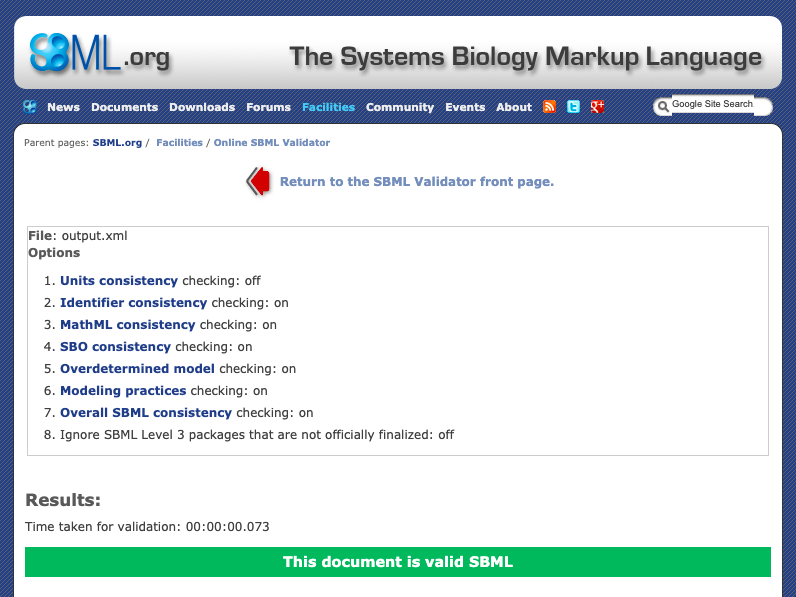
\includegraphics[scale=0.43]{images/example_validation.png}
\end{figure}

\lstinputlisting[language=xml, caption={File SBML in input \texttt{example.xml}}, label={lst:input.xml}]{../examples/input/example.xml}

\lstinputlisting[language=Turtle,linerange={219-271}, firstnumber=219, caption={Frammento del tile \texttt{output.ttl}, è stato omesso il preambolo per limitarne l'estensione}, label={lst:output.ttl}]{../examples/output/output.ttl}

\lstinputlisting[language=xml, caption={File SBML \texttt{output.xml} generato da \texttt{shacl2sbml.py}}, label={lst:output.xml}]{../examples/output/output.xml}

\clearpage
\section{Commenti e critiche}
Durante lo sviluppo del progetto si è tenuto conto dei seguenti commenti e critiche da parte del Professor Tronci:

\begin{longtable}{p{2cm}p{9cm}}
    \textbf{Data} & \textbf{Descrizione} \\
    \hline
    22/07/20 & Videochiamata con specifica del problema da parte del Professor Tronci. \\
    \hline
    27/07/20 & Prima stesura di una modellazione dei costrutti in SBML, avendo dimenticato di modellare extended SBML mi è stato fatto notare dal Professore e ho risolto, mi è stato anche consegnato il materiale su extended SBML da consultare. \\
    \hline
    28/07/20 & Corretto il punto precedente non avevo implementato deletion e replacement, il Professore ha inoltre consigliato la strategia di testing. \\
    \hline
    31/07/20 & Dopo aver aggiunto replacement e deletion e dopo aver eseguito dei test con risultati positivi è seguita una videochiamata con il Professor Tronci in cui mi è stato indicato di modificare il parser in maniera tale da poter ricevere in input più modelli SBML e di capire se il risultato di una query SPARQL rappresenti lo stesso tipo di conoscenza di un file XML/SBML, così da poter sfruttare questa corrispondenza per eseguire dei controtest. Questa corrispondenza esiste ed è usata spesso sotto il nome di "SPARQL query results xml format". \\
    \hline
    06/08/2020 & Videochiamata con il Professor Tronci in cui si è deciso di comprendere se fosse possibile scrivere un parser da SHACL a SBML e, in caso di risposta affermativa, farlo. \\
    \hline
    19/08/2020 & Correzioni su questa relazione ampliandola affinché i concetti risultino più chiari durante l'esposizione. \\
    \hline
    08/09/2020 & Videochiamata con il Professor Mancini nella quale si è esposto come la relazione mancasse di una componente didattica significativa. \\
    \hline
    15/09/2020 & Ulteriore videochiamata con il Professor Mancini perché l'estensione della relazione era ancora poco chiara. \\
    \hline
\end{longtable}

% bibliography
\clearpage
\phantomsection
%\addcontentsline{toc}{chapter}{\bibname}
%\bibliographystyle{sapthesis} % BibTeX style
%\bibliography{bibliography} % BibTeX database without .bib extension

\bibliographystyle{plainurl}
\bibliography{main}{}

\end{document}